%Compilation of research projects that we are interested in
\documentclass[11pt,compress,xcolor={usenames,dvipsnames},aspectratio=169]{beamer}
%\documentclass[xcolor={usenames,dvipsnames},aspectratio=169]{beamer} %slides and 
%notes
\usepackage[T1]{fontenc}
%\usepackage{tgadventor} %Font found at https://tug.org/FontCatalogue/
%\usepackage{newpxtext}
%\usepackage[euler-digits,euler-hat-accent]{eulervm}
\usepackage{xspace}


\usepackage{amsmath,
	amssymb,
	datetime,
	mathtools,
	bbm,
	%mathabx,
	array,
	booktabs,
	xspace,
	multirow,
	calc,
	colortbl,
	siunitx,
 	graphicx}
\usepackage{xcolor}
\usepackage[giveninits=false,backend=biber,style=authoryear, maxnames = 1000, maxcitenames = 10, mincitenames=9]{biblatex}
\addbibresource{FJHown25.bib}
\addbibresource{FJH25.bib}
\usepackage{media9}
\usepackage[autolinebreaks]{mcode}
\usepackage[tikz]{mdframed}


\usetheme{FJHSlimNoFoot169}
\setlength{\parskip}{2ex}
\setlength{\arraycolsep}{0.5ex}


\DeclareMathOperator{\SOL}{SOL}
\DeclareMathOperator{\APP}{APP}
\DeclareMathOperator{\ERR}{ERR}
\DeclareMathOperator{\AVG}{AVG}
\DeclareMathOperator{\INT}{INT}
\DeclareMathOperator{\LIN}{LINEAR}
\DeclareMathOperator{\BAD}{BAD}
%\DeclareMathOperator{\opt}{opt}
\newcommand{\dataN}{\bigl(\hf(\vk_i)\bigr)_{i=1}^n}
\newcommand{\dataNj}{\bigl(\hf(\vk_i)\bigr)_{i=1}^{n_j}}
\newcommand{\dataNjd}{\bigl(\hf(\vk_i)\bigr)_{i=1}^{n_{j^\dagger}}}
\newcommand{\ERRN}{\ERR\bigl(\dataN,n\bigr)}
\newcommand{\otod}{\ensuremath{1\mkern-4mu : \mkern-2mu d}}


%\DeclareMathOperator{\app}{app}

\providecommand{\HickernellFJ}{H.\xspace}


\renewcommand{\OffTitleLength}{-47ex}
\setlength{\FJHThankYouMessageOffset}{-8ex}
\title{Confidence Intervals for Quasi-Monte Carlo}
\author{
Aadit Jain\inst{1} \and
Fred J. Hickernell \inst{2} \and 
Aleksei G. Sorokin \inst{2,3}
}
\institute{
    \inst{1}Rancho Bernardo High School, San Diego, CA\\
	\inst{2}Department of Applied Mathematics \&
	Center for Interdisciplinary Scientific Computation \\
    Illinois Institute of Technology, Chicago, IL \qquad
	\href{mailto:hickernell@iit.edu}{\url{hickernell@iit.edu}} \\ 
    \inst{3} Sandia National Laboratory, Livermore, CA\qquad
	}

\thanksnote{Thanks to Art Owen and you all for the opportunity to discuss \\
Thanks to the Speedy Simulation Group, \href{http://qmcpy.org}{\nolinkurl{qmcpy.org}}}
	
%\event{Happy Fred}
\date[]{ revised \today}

\input FJHDef.tex



\begin{document}
	\everymath{\displaystyle}

\frame{\titlepage}

%%%%%%%%%%%%%%%%%%%%%%%%%%%%%%%%%%%%%%%%%%
%%%%%%%%%%%%%%%%%%%%%%%%%%%%%%%%%%%%%%%%%%
\section{Intro}
%%%%%%%%%%%%%%%%%%%%%%%%%%%%%%%%%%%%%%%%%%
%%%%%%%%%%%%%%%%%%%%%%%%%%%%%%%%%%%%%%%%%%

\begin{frame}{Questions}

\vspace{-6ex}
Given $\{Y_i =  f(\vX_i)\}_{i=0}^{\infty}$, how can one construct reasonable confidence intervals
\begin{equation*}
    \Prob \Bigl [\Bigl \lvert\underbrace{\Ex(Y)}_{\mu} - \underbrace{\frac{1}{n} \sum_{i=0}^{n-1} Y_i}_{\hmu_n}  \Bigr \rvert \le \varepsilon \Bigr ] \ge 1 - \alpha
\end{equation*}

\begin{itemize}
\item Are these intervals good for just a particular $n$ (confidence intervals, CIs) or all $n$ (confidence sequences, CSs)

\item What if the $\{\vX_i\}_{i=0}^{\infty}$ are not independent and identically distributed (IID), such as coming from quasi-Monte Carlo (QMC), aka low discrepancy (LD) sequences?

\item What kind of additional information on $f$ is needed or might be helpful?
\end{itemize}

   
\end{frame}


\begin{frame}{Known confidence intervals}

\vspace{-6ex}

\cite{BahSav56} established that nonparametric tests cannot achieve the same efficiency as parametric tests for convex, balanced sets of random variables

\begin{description}
    \item[Chebyshev] $\Prob \Big[\abs{\mu - \hmu_n} \ge \frac{\std(Y)}{\sqrt{\alpha n}} \Bigr] \le 1 - \alpha$  for IID $Y_0, Y_1, \ldots$

    \item[Central Limit Theorem(CLT)]
    $\Prob \Big[\abs{\mu - \hmu_n} \le \frac{\std(Y) \Phi^{-1}(1 -  \alpha/2)}{\sqrt{n}} \Bigr] \approx 1 - \alpha$  for IID $Y_0, Y_1, \ldots$ as $n \to \infty$

    \item[Berry-Esseen] Generalizes CLT; \textcite{HicEtal14a} derived guaranteed CIs  for functions of bounded kurtosis

    \item[Others] Hoeffding, Bernstein 
\end{description}
   
\end{frame}



\begin{frame}{Known confidence sequences}

 \vspace{-5ex}
\begin{tabular}
    {
    >{\raggedright\small}p{0.2\textwidth} 
    >{\raggedright\small}p{0.2\textwidth}
    >{\raggedright\small}p{0.25\textwidth} 
    >{\raggedright\small}p{0.25\textwidth}
    }
        \textbf{Method} & \textbf{Assumes} & \textbf{Strengths} & \textbf{Weaknesses} \tabularnewline
        \toprule
        Bernstein CS & Bounded $Y \in [a,b]$, variance known & Adapts to variance when known & Requires prior knowledge of variance \tabularnewline
        \midrule
        Empirical Bernstein CS & Bounded $Y \in [a,b]$, variance estimated & Adapts to variance, improves on Hoeffding & Slightly more complex, slower early shrinkage \\
        \tabularnewline
        \midrule
        Supermartingale-Based CS \parencite{HowEtal21a} & Independent observations, no parametric assumptions & Generalizes many CSs, works with sequential data & Requires martingale-based setup \tabularnewline
        \midrule
        Betting-Based CS \parencite{WauRam24a} & Bounded $Y \in [a,b]$, sequential setting & Tightest known CS, variance-adaptive, allows flexible stopping & More complex, requires good betting strategy \tabularnewline
        \bottomrule
    \end{tabular}

\end{frame}

\section{Quasi-Monte Carlo}
\begin{frame}{Quasi-Monte Carlo \href{https://qmcpy.org}{\nolinkurl{qmcpy.org}} fills space more evenly}

\begin{itemize}
    \item Deterministic (100\%) confidence intervals for $f$ in cones of functions whose Fourier complex exponential / Walsh coefficients decay reasonably using latttices / digital nets \parencite{HicJim16a, JimHic16a, HicEtal17a,JagSor23a}

    \item Bayesian credible intervals using $\Order(n \log n) $ operations for lattices / digital nets with well-fitting covariance kernels \parencite{RatHic19a,JagHic22a}

    \item See Art and others \parencite{LEcEtal24a,Owe26a}
\end{itemize}
    
\end{frame}

\section{Betting CIs/CSs with QMC}
\begin{frame}{Numerical Experiments}
\vspace{-15ex}
 \begin{align*}
    n &= \text{number of LD samples per replication}\\
    R & = \text{number of IID replications} \\
    N & = \text{total number of samples} = nR
\end{align*} 
What is the optimal ratio of $n$ to $R$?
\end{frame}

\begin{frame}{Beta Distribution}

\vspace{-7ex}

Example from \textcite{WauRam24a} ($n=32$, $R =100$)

\centerline{
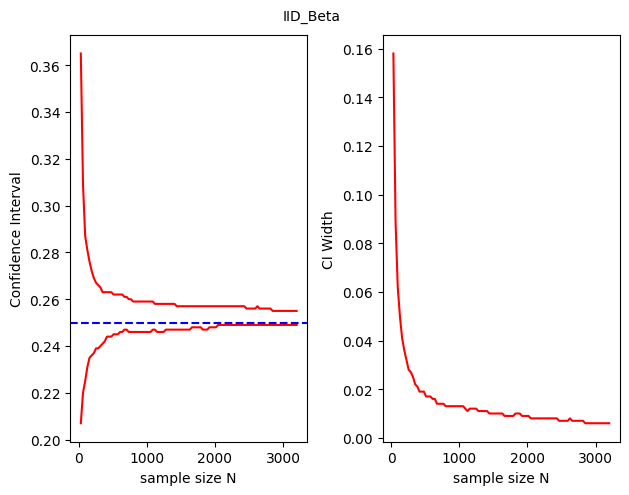
\includegraphics[width=0.45\textwidth]{Figures/IID_Beta.png} \qquad
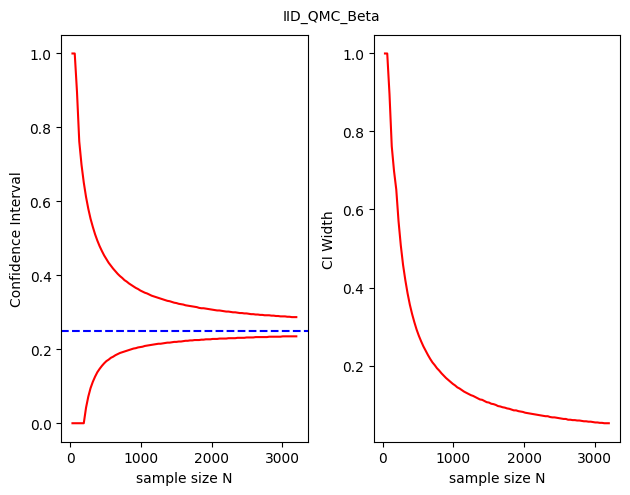
\includegraphics[width=0.45\textwidth]{Figures/IID_QMC_Beta.png} }
    
\end{frame}

\begin{frame}{Beta Distribution cont'd}
\vspace{-7ex}

$N = 1024$
\centerline{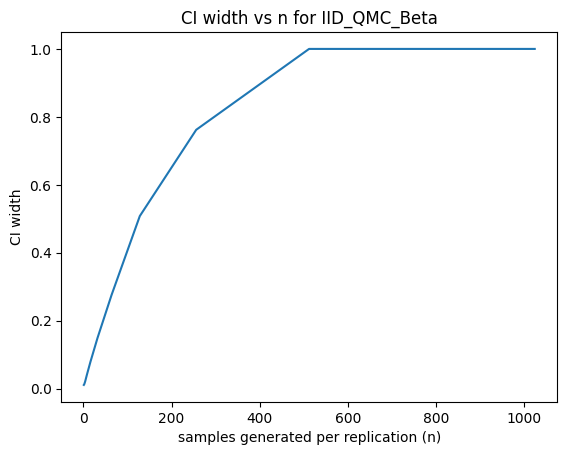
\includegraphics[width=0.5\textwidth]{Figures/beta_vary.png}}
    
\end{frame}

\begin{frame}{Univariate Exponential}
\vspace{-7ex}
\[
f(x) = x\exp(x-1), \quad x \in [0,1], \qquad N = 1024
\]
\centerline{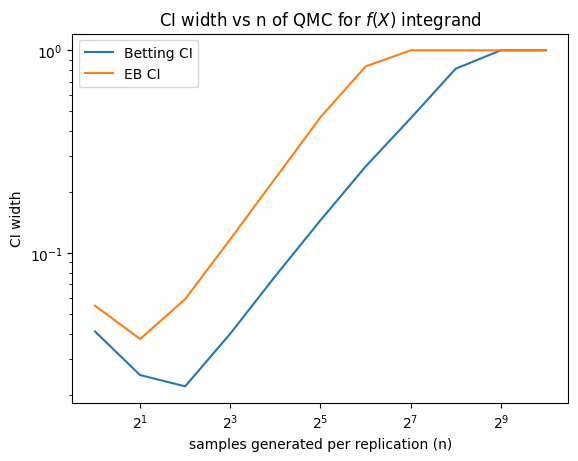
\includegraphics[width=0.45\textwidth]{Figures/f(x).png}
\quad
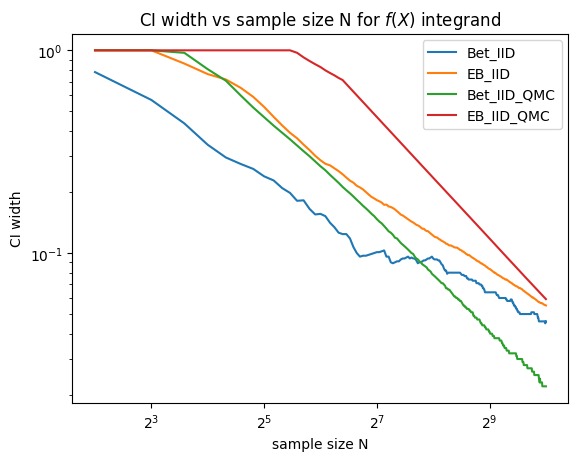
\includegraphics[width=0.45\textwidth]{Figures/f(x)_opt_n.png}} 

\vspace{-3ex}
\hspace{0.72\textwidth}$n=4$
    
\end{frame}

\begin{frame}{Bivariate Discontinuous}
\vspace{-7ex}
\[
f(x_1,x_2) = \bbone_{[2/3,2]}(x_1+x_2), \quad x_1,x_2 \in [0,1]
\]
\centerline{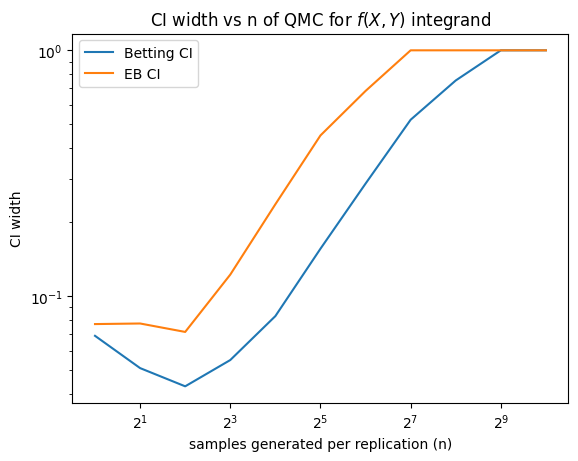
\includegraphics[width=0.45\textwidth]{Figures/f(x,y).png}
\quad
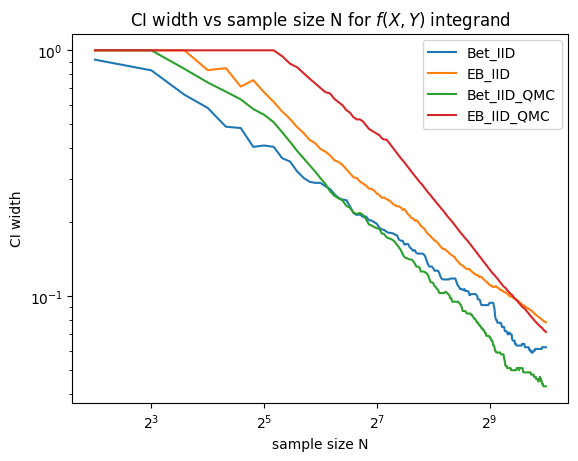
\includegraphics[width=0.45\textwidth]{Figures/f(x,y)_opt_n.png}} 
    
\end{frame}



\begin{frame}{Ridge Functions}

$N = 1024$

\vspace{-10ex}

\centerline{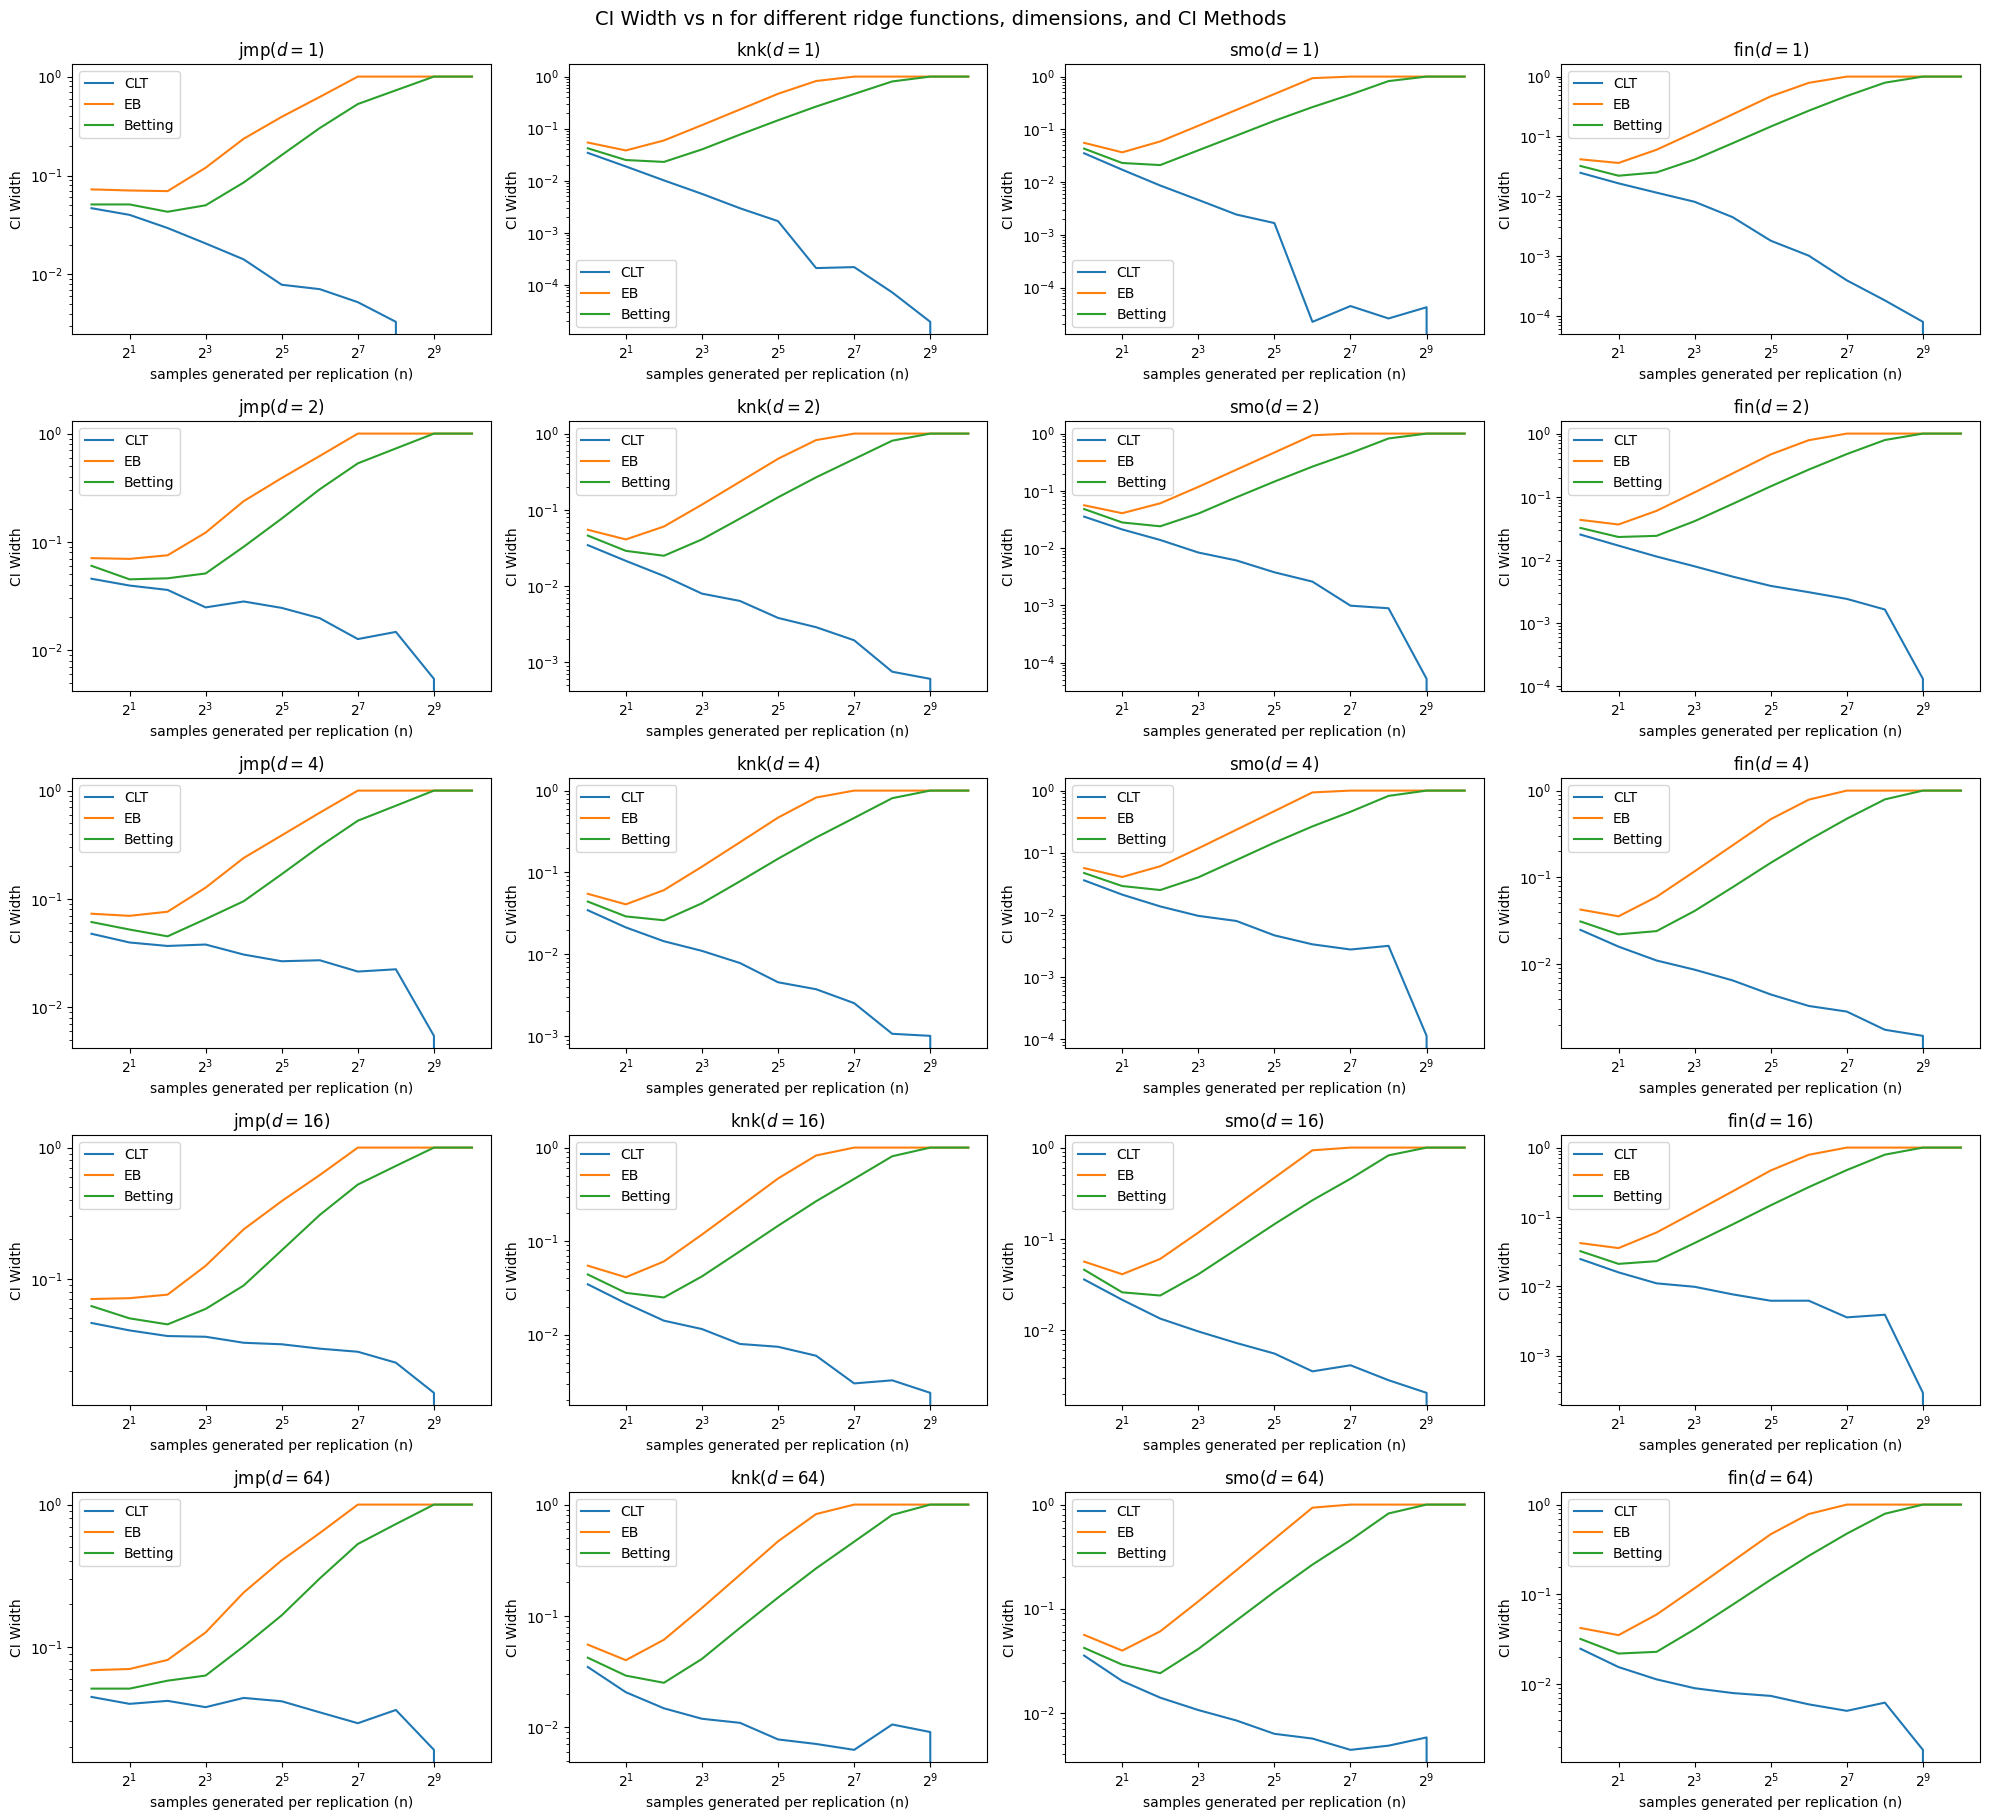
\includegraphics[width=0.6\textwidth]{Figures/ridge.png}}
    
\end{frame}



\begin{frame}[allowframebreaks]{References}
\printbibliography
\end{frame}




\end{document}